\documentclass[main.tex]{subfiles}
\begin{document}
设一混合物系统的某广度性质$M$是状态函数,不妨记作$M=M\left(X,Y,\left\{n_i\right\}\right)$,其中$X$、$Y$表示除组成$\left\{n_i\right\}$外,独立、完整确定系统状态的其他强度性质。组份$i$在系统中的\emph{偏摩尔性质(partial molar properties)}定义为\footnote{大部分资料中的偏摩尔量定义规定为$X=T$、$Y=p$的情况,但这并不是必要的。我们将看到,推广为一般情况并不增加难度,且所有偏摩尔量的规律仍成立。本节的推导过程是跟《物理化学》\S4.3很像的。}
\[M_i\eqdef\left.\frac{\partial M}{\partial n_i}\right|_{X,Y,\left\{n_{j\neq i}\right\}}\]
表\ref{tab:molar_partial_molar_notaion}还列出了其他混合物性质的定义,同时给出了它们在本讲义中的记号惯例。

\begin{longtable}{p{0.25\textwidth}p{0.3\textwidth}p{0.3\textwidth}}
  \caption{各种摩尔量和偏摩尔量的符号和定义}\label{tab:molar_partial_molar_notaion}                                                                                                    \\
  \hline
  $M\left(X,Y,\left\{n_i\right\}\right)$                         & 混合物的某广度性质        &                                                                                  \\
  $M_\text{m}\left(X,Y,\left\{n_i\right\}\right)$                & 混合物的摩尔性质         & $M_\text{m}\eqdef M/n$                                                           \\
  $M_i\left(X,Y,\left\{n_j\right\}\right)$                       & 组份$i$在混合物中的偏摩尔性质 & $M_i\eqdef\left(\partial M/\partial n_i\right)_{X,Y,\left\{n_{j\neq i}\right\}}$ \\
  $M_{\text{m},i}^*\left(X,Y\right)\equiv M_i^*\left(X,Y\right)$ & 组份$i$纯物质的(偏)摩尔性质 & $M_i^*\left(X,Y,n_i\right)$,按上列定义计算。                                             \\
  \hline
\end{longtable}

偏摩尔热力学函数之间的关系,跟总热力学函数的形式一样。这是可以通过Tobolsky方法推出来的。例如,取$\left(T,p,\left\{n_i\right\}\right)$为状态变量,由$U=U\left(T,p,\left\{n_i\right\}\right)$,
\[\mathrm{d}U=\left.\frac{\partial U}{\partial T}\right|_{p,\left\{n_i\right\}}\mathrm{d}T+\left.\frac{\partial U}{\partial p}\right|_{T,\left\{n_i\right\}}\mathrm{d}p+\sum_i U_i\mathrm{d}n_i\]
按照Tobolsky方法,我们由式\eqref{eq:I.1_first_law_multicomp}出发,把$\mathrm{d}S$和$\mathrm{d}V$换成$\mathrm{d}T$和$\mathrm{d}p$。由$S=S\left(T,p,\left\{n_i\right\}\right)$和式\eqref{eq:I.1_Maxwell_GTp}有:
\[\mathrm{d}S=\frac{C_p}{T}\mathrm{d}T-V\alpha_p\mathrm{d}p+\sum_iS_i\mathrm{d}n_i\]
由$V=V\left(T,p,\left\{n_i\right\}\right)$(即系统的$pVTn_i$状态方程)有:
\[\mathrm{d}V=V\alpha_p\mathrm{d}T-V\kappa_T\mathrm{d}p+\sum_in_iV_i\]
代入式\eqref{eq:I.1_first_law_multicomp}得
\[\mathrm{d}U=\left(C_p-pV\alpha_p\right)\mathrm{d}T+\left(pV\kappa_T-TV\alpha_p\right)\mathrm{d}p+\sum_i\left(\mu_i+TS_i-pV_i\right)\mathrm{d}n_i\]
与$U\left(T,p,\left\{n_i\right\}\right)$的全微分比较可得:
\begin{equation}\label{eq:II.2_partial_molar_thermodynamic_functions_relation}
  \mu_i=U_i+pV_i-TS_i
\end{equation}
留意到$\mu_i\equiv G_i$,可见上式的定义跟吉布斯自由能本身的定义形式是一模一样的。这将使得第\ref{sec:I_thermodynamic_relations}章推导的那些关于$U$、$S$、$H$、$A$和$G$之间的各种热力学关系式——\eqref{eq:I.1_first_law_multicomp}至\eqref{eq:I.1_dG}、式\eqref{eq:I.1_first_order_partial_T}至\eqref{eq:I.1_heat_capacity_entropy_V},以及表\ref{tab:Maxwell_relations},式\eqref{eq:I.1_dS_T_V}和\eqref{eq:I.1_dS_T_p}——对于它们的偏摩尔量也适用,只需把这些关系式里面凡是广度性质都换成偏摩尔性质即可。应用Tobolsky方法还能把这些偏摩尔量相应地表示成式\eqref{eq:I.1_def_Cpi}至\eqref{eq:I.1_def_partial_molar_compressibility}定义的偏摩尔响应函数的形式。需要注意的是,$\mu_i$本身是哪个热力学势的偏摩尔量,依状态变明$X$、$Y$的选取而定(见式\eqref{eq:I.1_first_order_partial_mu})。例如,若取$\left(T,V,\left\{n_i\right\}\right)$为状态变量情况,我们仍说“偏摩尔热力学函数之间的关系,跟总热力学函数的形式一样”这句话,但$mu_i$要当作亥姆霍兹自由能的偏摩尔量来看待。

仅由偏摩尔量的定义和热力学基本关系,还可推出两个重要知识:偏摩尔量的加和性和吉布斯--杜安方程。

\subsection{偏摩尔量的加和性}
在本小节我们将证明
\begin{equation}\label{eq:II.2_additivity_partial_molar_quantity_1}
  M=\sum_in_iM_i
\end{equation}
定义混合物系统的\emph{摩尔量(molar porperties)}为
\[M_\text{m}\eqdef \frac{M}{n}\]
则式\eqref{eq:II.2_additivity_partial_molar_quantity_1}又可写成
\begin{equation}\label{eq:II.2_additivity_partial_molar_quantity_2}
  M_\text{m}=\sum_ix_iM_i
\end{equation}
这件事称为偏摩尔量的加和性。由此可知,摩尔量和偏摩尔量(包括化学势)都是强度性质。

值得注意的是,摩尔量也满足第\ref{sec:I_thermodynamic_relations}章推导的那些关于$U$、$S$、$H$、$A$和$G$之间的各种热力学关系式——\eqref{eq:I.1_first_law_multicomp}至\eqref{eq:I.1_dG}、式\eqref{eq:I.1_first_order_partial_T}至\eqref{eq:I.1_heat_capacity_entropy_V},以及表\ref{tab:Maxwell_relations},式\eqref{eq:I.1_dS_T_V}和\eqref{eq:I.1_dS_T_p}——只需把这些关系式中的广度性质全部换成摩尔量即可。以下以吉布斯自由能为例证明式\eqref{eq:I.1_dG}对摩尔吉布斯自由能的适用性。从以下微分出发,并作相应的偏导数,不难得到
\begin{align*}
  \mathrm{d}G_\text{m} & =\mathrm{d}\left(G/n\right)=\left.\frac{\partial\left(G/n\right)}{\partial T}\right|_{p,\left\{n_i\right\}}\mathrm{d}T+\left.\frac{\partial\left(G/n\right)}{\partial p}\right|_{T,\left\{n_i\right\}}\mathrm{d}p+\sum_i\left.\frac{\partial\left(G/n\right)}{\partial n_i}\right|_{T,p,\left\{n_{j\neq i}\right\}}\mathrm{d}n_i \\
                       & =-S_\text{m}\mathrm{d}T+V_\text{m}\mathrm{d}p+\sum_i\left(\mu_i-G_\text{m}\right)\mathrm{d}x_i                                                                                                                                                                                                                                   \\
                       & =-S_\text{m}\mathrm{d}T+V_\text{m}\mathrm{d}p+\sum_i\mu_i\mathrm{d}x_i
\end{align*}
其中用到条件$\sum_i\mathrm{d}x_i\equiv 0$。

以下简单证明偏摩尔量的加和性。由广度性质的定义可知, $M$与$n\equiv\sum_in_i$成正比。故对每一$X$、$Y$有
\[M\left(X,Y,\left\{\lambda n_i\right\}\right)=\lambda M\left(X,Y,\left\{n_i\right\}\right)\]
其中$\lambda$为任意正实数。该性质又可说成是:混合物系统的广度性质,是系统各组份摩尔数的1次齐函数\footnote{见《物理化学》附录I.8,或者\S\ref{sec:A.1_Euler_theorem_homogeneous_function}。}。由欧拉齐函数定理可直接得到偏摩尔量的加和性结论。

式\eqref{eq:II.2_additivity_partial_molar_quantity_2}又可以这样推导。由全微分式
\[\mathrm{d}M=\left.\frac{\partial M}{\partial X}\right|_{Y,\left\{n_i\right\}}\mathrm{d}X+\left.\frac{\partial M}{\partial Y}\right|_{X,\left\{n_i\right\}}\mathrm{d}Y+\sum_i M_i\mathrm{d}n_i\]
和以下系列微分关系式
\begin{align*}
  \mathrm{d}M                                                       & =\mathrm{d}\left(nM_\text{m}\right)=n\mathrm{d}M_\text{m}+M_\text{m}\mathrm{d}n                                                                                       \\
  \mathrm{d}n_i                                                     & =\mathrm{d}\left(x_i n\right)=x_i\mathrm{d}n_i+n\mathrm{d}x_i                                                                                                         \\
  \left.\frac{\partial M}{\partial X}\right|_{Y,\left\{n_i\right\}} & =\left.\frac{\partial \left(nM_\text{m}\right)}{\partial X}\right|_{Y,\left\{n_i\right\}}=n\left.\frac{\partial M_\text{m}}{\partial X}\right|_{Y,\left\{x_i\right\}} \\
  \left.\frac{\partial M}{\partial Y}\right|_{Y,\left\{n_i\right\}} & =\left.\frac{\partial\left(nM_\text{m}\right)}{\partial Y}\right|_{X,\left\{n_i\right\}}=n\left.\frac{\partial M_\text{m}}{\partial Y}\right|_{X,\left\{x_i\right\}}
\end{align*}
可得
\begin{align*}
    & n\left(\mathrm{d}M_\text{m}-\left.\frac{\partial M_\text{m}}{\partial X}\right|_{Y,\left\{x_i\right\}}\mathrm{d}X-\left.\frac{\partial M_\text{m}}{\partial Y}\right|_{X,\left\{x_i\right\}}\mathrm{d}Y-\sum_iM_i\mathrm{d}x_i\right) \\
  + & \left(M_\text{m}-\sum_ix_iM_i\right)\mathrm{d}n=0
\end{align*}
上式第一项恰好就是$M$的全微分式,故为零。剩下的含$\mathrm{d}n$的一项也只能为零,得到式\eqref{eq:II.2_additivity_partial_molar_quantity_2}。

\subsection{吉布斯--杜安方程}
由偏摩尔量的加和性,联系$M$的全微分式
\begin{align*}
  \mathrm{d}M & =\mathrm{d}\left(\sum_in_iM_i\right)=\sum_in_i\mathrm{d}M_i+\sum_iM_i\mathrm{d}n_i                                                                                                \\
              & =\left.\frac{\partial M}{\partial X}\right|_{Y,\left\{n_i\right\}}\mathrm{d}X+\left.\frac{\partial M}{\partial Y}\right|_{X,\left\{n_i\right\}}\mathrm{d}Y+\sum_iM_i\mathrm{d}n_i
\end{align*}
可得到下式
\begin{equation}\label{eq:II.2_Gibbs_Duhem_eq}
  \sum_in_i\mathrm{d}M_i=\left.\frac{\partial M}{\partial X}\right|_{Y,\left\{n_i\right\}}\mathrm{d}X+\left.\frac{\partial M}{\partial Y}\right|_{X,\left\{n_i\right\}}\mathrm{d}Y
\end{equation}
该式称\emph{吉布斯--杜安方程(Gibbs--Duhem equation)}。它在$X$、$Y$恒定条件下的形式是
\begin{equation}\label{eq:II.2_Gibbs_Duhem_eq_XYConst}
  \sum_in_i\mathrm{d}M_i=0
\end{equation}
《物理化学》书上的吉布斯--杜安方程只是$M=G$、$X=T$、$Y=p$的特例而已:
\begin{equation}\label{eq:II.2_Gibbs_Duhem_eq_for_G}
  \sum_in_id\mu_i=-S\mathrm{d}T+V\mathrm{d}P
\end{equation}
其中用到了式\eqref{eq:I.1_first_order_partial_mu}、\eqref{eq:I.1_first_order_partial_V}和\eqref{eq:I.1_first_order_partial_S}。


\subsection{不同状态变量下的偏摩尔量之间的关系}
对于同一系统,采用不同的两组状态变量——
\[\left(X,Y,\left\{n_i\right\}\right)\text{和}\left(X^\prime,Y^\prime,\left\{n_i\right\}\right)\]
下,$M\left(X,Y,\left\{n_i\right\}\right)$和$M\left(X^\prime, Y^\prime,\left\{n_i\right\}\right)$一般是不同表达式的函数,因此在相应条件下定义的偏摩尔量也是不同表达式的函数。若我们小心地将同一系统在第二组状态参数$\left(X^\prime,Y^\prime,\left\{n_i\right\}\right)$下的同一性质另记为
\[M^\prime\equiv M^\prime\left(X^\prime,Y^\prime,\left\{n_i\right\}\right)\]
则如下所示$M_i$与$M_i^\prime$是相互联系的。

由于系统的平衡状态是唯一的,使系统处于相同状态的一对状态参数$\left(X,Y,\left\{n_i\right\}\right)$和$\left(X^\prime,Y^\prime,\left\{n_i\right\}\right)$取值之间是一一对应的。由$M$的全微分式,
\[\mathrm{d}M=\left.\frac{\partial M}{\partial X}\right|_{Y,\left\{n_i\right\}}\mathrm{d}X+\left.\frac{\partial M}{\partial Y}\right|_{X,\left\{n_i\right\}}\mathrm{d}Y+\sum_i M_i\mathrm{d}n_i\]
两边除以$\mathrm{d}n_i$,保持$X^\prime$、$Y^\prime$恒定,可得
\[M_i^\prime=\left.\frac{\partial M}{\partial X}\right|_{Y,\left\{n_i\right\}}\left.\frac{\partial X}{\partial n_i}\right|_{X^\prime,Y^\prime,\left\{n_{j\neq i}\right\}}+\left.\frac{\partial M}{\partial Y}\right|_{X,\left\{n_i\right\}}\left.\frac{\partial Y}{\partial n_i}\right|_{X^\prime,Y^\prime,\left\{n_{j\neq i}\right\}}+M_i\]
此即为$M_i^\prime$与$M_i$之间的一般关系式。所用到的两个偏微分——
\[\left.\frac{\partial X}{\partial n_i}\right|_{X^\prime,Y^\prime,\left\{n_{j\neq i}\right\}},\quad\left.\frac{\partial Y}{\partial n_i}\right|_{X^\prime,Y^\prime,\left\{n_{j\neq i}\right\}}\]
是由混合物系统的状态方程可知的。例如,我们要考虑$\left(T,p,\left\{n_i\right\}\right)$和$\left(T,V\left\{n_i\right\}\right)$下定义的偏摩尔量之间的关系,那就是
\begin{align*}
  \left.\frac{\partial M}{\partial n_i}\right|_{T,V,\left\{n_{j\neq i}\right\}} & =\left.\frac{\partial M}{\partial p}\right|_{T,\left\{n_i\right\}}\left.\frac{\partial p}{\partial n_i}\right|_{T,V,\left\{n_{j\neq i}\right\}}+\left.\frac{\partial M}{\partial n_i}\right|_{T,p,\left\{n_{j\neq i}\right\}} \\
  \left.\frac{\partial M}{\partial n_i}\right|_{T,p,\left\{n_{j\neq i}\right\}} & =\left.\frac{\partial M}{\partial V}\right|_{T,\left\{n_i\right\}}\left.\frac{\partial V}{\partial n_i}\right|_{T,p,\left\{n_{j\neq i}\right\}}+\left.\frac{\partial M}{\partial n_i}\right|_{T,V,\left\{n_{j\neq i}\right\}}
\end{align*}
可见,要作两种偏摩尔性质之间的转换计算需已知混合物的状态方程,以便求得以下两个偏导数
\[\left.\frac{\partial p}{\partial n_i}\right|_{T,V,\left\{n_{j\neq i}\right\}},\quad\left.\frac{\partial V}{\partial n_i}\right|_{T,p,\left\{n_{j\neq i}\right\}}\]
这两个偏导数在第\ref{sec:I_thermodynamic_relations}章已经讨论过了,都属于可测量。

\subsection{偏摩尔量的测定}
实验上,我们往往只能测量一个多组份系统的摩尔量$M_\text{m}=M_\text{m}\left(X,Y,\left\{n_i\right\}\right)$随某组份$i$在恒定$X$、$Y$下的变化。以下推算,使得我们能够通过$M_\text{m}$对$x_i$的曲线得出$M_i$。

在恒定$X$、$Y$下,$M=n M_\text{m}$,对其进行微分有
\[\mathrm{d}\left(nM_\text{m}\right)=n\mathrm{d}M_\text{m}+M_\text{m}\mathrm{d}n\]
对$n=\sum_i n_i$进行微分有
\[\mathrm{d}n=\sum_i\mathrm{d}n_i\]
上列两式联立起来有
\[n\mathrm{d}M_\text{m}+M_\text{m}\sum_i \mathrm{d}n_i=\sum_i M_i\mathrm{d}n_i\]
利用该式求关于$n_i$的偏导(即保持$\left\{n_{j\neq i}\right\}$恒定),得到
\begin{align*}
                  & n\left.\frac{\partial M_\text{m}}{\partial n_i}\right|_{X,Y,\left\{n_{j\neq i}\right\}}+M_\text{m}=M_i+\sum_{j\neq i}M_j\left.\frac{\partial n_j}{\partial n_i}\right|_{n_{j\neq i}} \\
  \Leftrightarrow & \left(1-x_i\right)\left.\frac{\partial M_\text{m}}{\partial x_i}\right|_{X,Y,\left\{n_{j\neq i}\right\}}+M_\text{m}=M_i
\end{align*}

利用这一结论,偏摩尔量$M_i$就能由摩尔量$M_\text{m}$对$x_i$的曲线数据,如图\ref{fig:meas_partial_molar_quant}所示般得出。

\begin{figure}[ht]
  \centering
  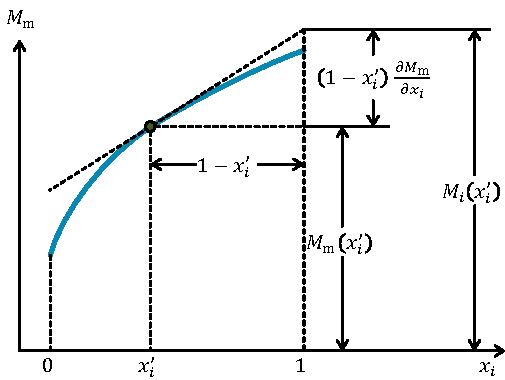
\includegraphics{../images/meas_partial_molar_quant.pdf}
  \caption{从摩尔量曲线求偏摩尔量的“截距法”。}
  \label{fig:meas_partial_molar_quant}
\end{figure}

《物理化学》\S 4.3中的“偏摩尔量的求法”之“3.截距法”介绍了上述方法对于双组份混合物的特例。
\end{document}